
Memory allocation in the VM is extremely important because there is a need to
repeatedly allocate and deallocate logical facts. Logical facts tend to be small
memory objects, requiring, on average, 24 to 30 bytes of memory, which may lead
to fragmentation if allocation is not done carefully.  Moreover, since VM is
multithreaded, allocation also needs to be scalable, therefore using the
standard \code{malloc} facility provided by the POSIX standard may not be the
best idea since each operating system uses a different implementation that may
or may scale well in multithreaded environments.

\begin{figure}[ht]
   \begin{center}
      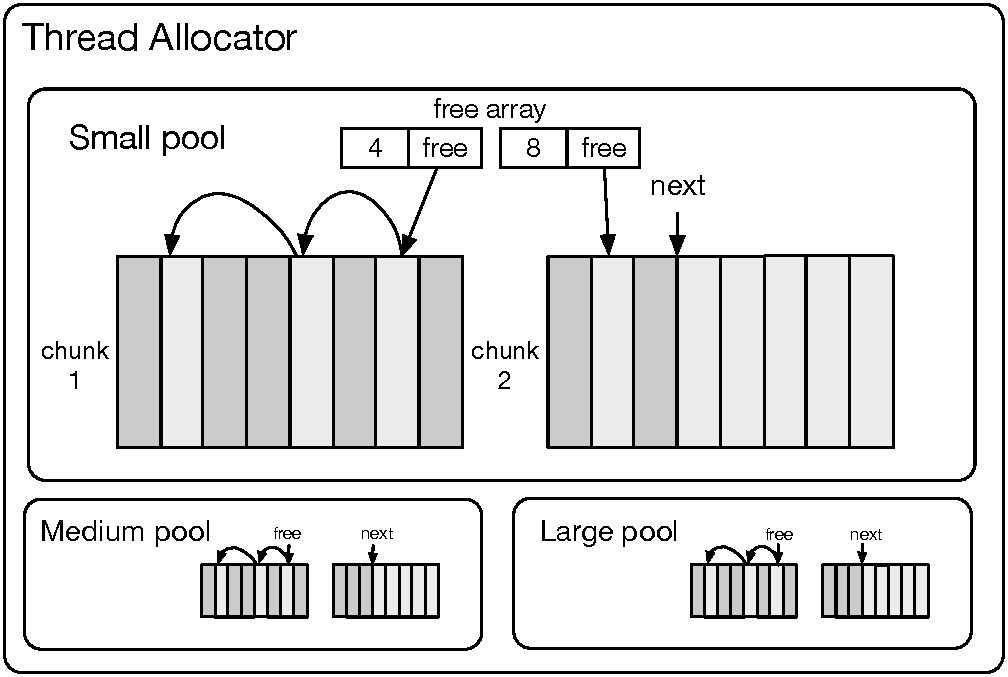
\includegraphics[width=0.7\linewidth]{figures/implementation/pool.pdf}
   \end{center}
   \caption{Thread allocator: each thread has a pool of slabs for allocating
      data structures. Each object size has: (1) several slabs that store contiguous chunks of
      memory of the same size; (2) a free list \code{free} of chunks that were freed; and (3) a \code{next} pointer that points to the next available free chunk.}
   \label{fig:implementation:pool}
\end{figure}

In order to solve these two issues, we decided to implement an allocator based
on the SLAB allocator~\cite{Bonwick-94}. SLAB allocation is a memory management
technique created in the Solaris 5.4 kernel used for efficiently allocate kernel
objects. Its advantages include reduced fragmentation and improved reuse of
deallocated data structures since these are reused in newer allocations.

Our particular implementation is presented in Fig.~\ref{fig:implementation:pool}
We pre-allocate multiple pools of memory chunks. We create one pool per object
size or data structure and each pool allocates large contiguous chunks of memory
that contain multiple objects of the same size. When allocating a particular
data structure, we first lookup the pool that
handles objects of the fact size and then check if there is an available object
in the chunks of memory. If all the chunks are empty, we use the \code{next}
pointer to allocate a new object inside a chunk. If there is no available space
in the chunk pointed by \code{next}, then we allocate a bigger chunk. We also
have a pointer \code{free} that points to deallocate objects and which creates a
list of free objects inside the available chunks. If the list has free objects,
we use the object pointed by \code{free} and update the \code{free} pointer
accodingly.

In order to reduce thread contention in the allocator, each thread uses a
different instance of the threaded allocator. When a thread wants to allocate an
object, it asks its own allocator for a new object. When deallocating, a thread
may deallocate an object that is part of another thread's allocator. However,
this is not an issue since chunks are not garbage collected from the system,
which allows another thread to reuse the pointer for a later allocation.

\iffalse
\subsection{Fact Allocation}

Although threads only allocate from their own memory chunks, they may reuse
objects from chunks created by another thread. Consider the following sequence
of events: (1) thread \code{T1} allocates multiple facts for node \code{A} in
the memory chunk \code{C1}; (2) thread \code{T2} executes node \code{A} and
allocates several facts in its own memory chunk \code{C2}; (3) thread \code{T1}
executes \code{A} again and needs to iterate through \code{A}'s facts which are
located in different multiple chunks, resulting in poor memory locality and
increased cache line misses. It is obvious that, in a perfect scenario,
\code{A}'s facts should be placed in a contiguous memory area in order to reduce
cache misses.

To tackle these issues, we have implemented a per-node fact allocator that is
implemented on top of the threaded allocator. The fact allocator allocates
chunks of memory from the main allocator which are then used to allocate facts
for that particular node. When a thread needs to allocate or deallocate a fact,
it acquires the allocator lock of the target node's allocator and performs the
allocation operation. Each fact allocator can allocate multiple chunks of
memory, depending on the amount of required facts. There is a doubly-linked list
of memory chunks and each chunk contains facts of different sizes (predicates).

Figure~\ref{fig:implementation:fact_allocator} presents an example state of a
fact allocator. The node has 3 memory chunks, all connected using the
\code{next} and \code{prev} pointers. Each chunk also has a reference count
(\code{refcount}) of the facts allocated in the chunk. If the reference count
ever drops to zero, then the memory chunk is deallocated. Deallocated facts are
kept on an array of linked lists named \code{free\_list} (contiguous in the
chunk, not as separate data structure), where each position of the array is a
linked list for facts with the same size. When allocating a new fact, we use the
first element of the linked list for facts with the same size.

\begin{figure}[ht]
   \begin{center}
      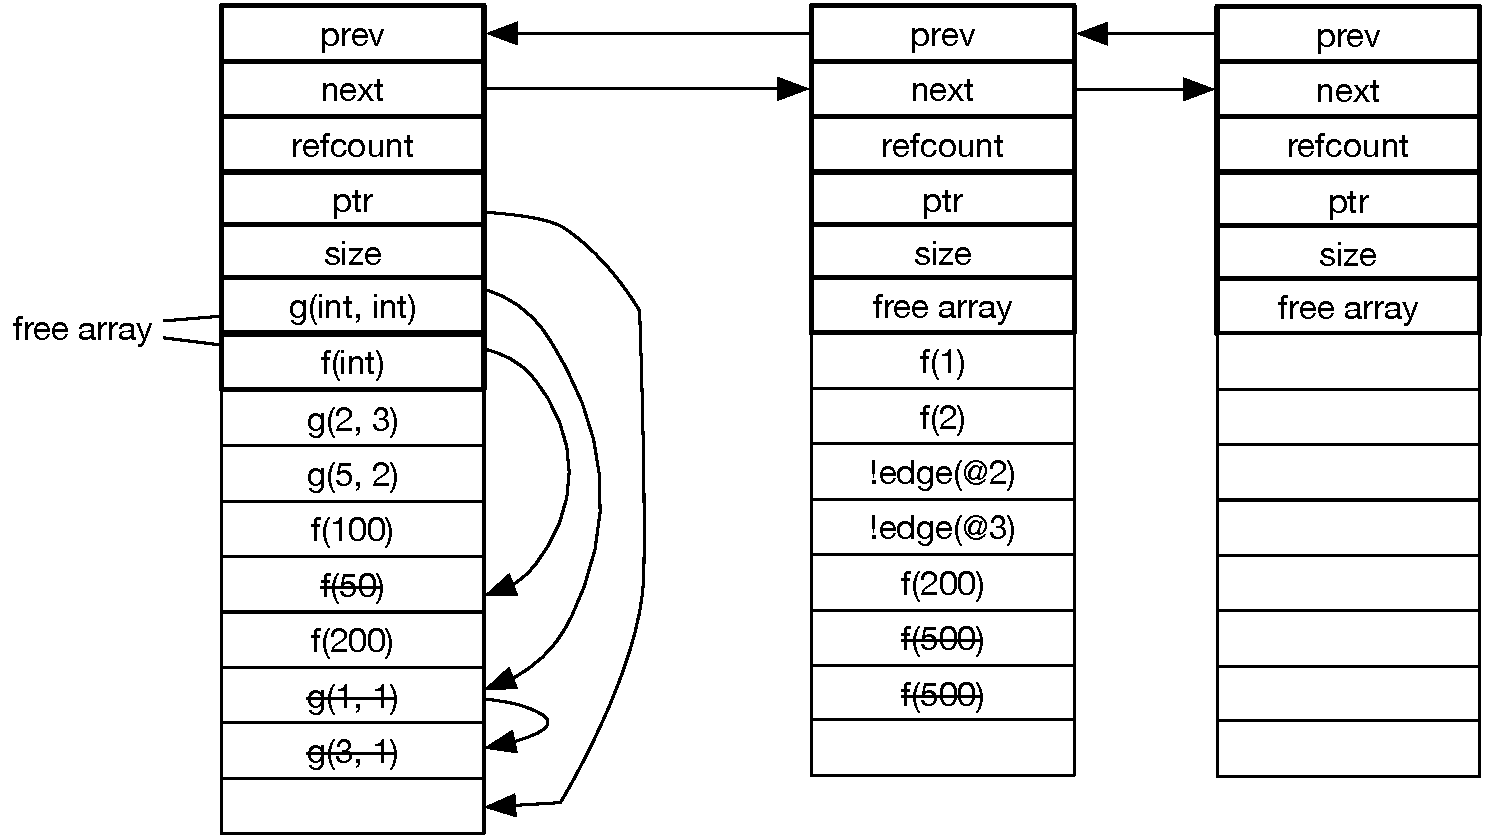
\includegraphics[width=0.7\linewidth]{figures/implementation/fact_allocator.pdf}
   \end{center}
   \caption{Fact allocator: each node has a pool of memory chunks for allocating
      logical facts. Each chunk contains: (1) several linked lists of free facts
      of the same size (\code{free\_list}); (2) a reference count of used facts
      (\code{refcount}); (3) a \code{ptr} pointer that points to unallocated
      space in the chunk. In this figure, predicates \code{f} and \code{g} have
   several deallocated facts that are ready to be used when a new fact needs to
be acquired.}
   \label{fig:implementation:fact_allocator}
\end{figure}
\fi
